\documentclass[a4paper, 10pt]{report}
\usepackage[italian]{babel}
\usepackage[T1]{fontenc}
\usepackage[utf8]{inputenc}
\usepackage{charter}
\usepackage{amsmath}
\usepackage{amsthm}
\usepackage{amsfonts}
\usepackage{graphicx}
\usepackage{wrapfig}
\usepackage{tcolorbox}
\usepackage{fancyhdr}
\usepackage{listings}

\usepackage{geometry}
\geometry{a4paper, left=2cm,right=2cm,top=2cm,bottom=2cm}

\pagestyle{fancy}
\lhead{}
\chead{}
\rhead{\bfseries 15 ottobre 2019 }
\lhead{\bfseries Linguaggi}

\begin{document}

\subsection*{Semantica (pt. 2)}

Poichè il significato di un programma può essere guardato da punti di vista diversi, si sono sviluppate diverse tipologie di analisi semantica:
\begin{itemize}
\item[-] Semantica denotazionale: descrive le funzionalità studiando gli effetti dell'esecuzione e cercando le proprietà del programma a partire da quelle della funzione calcolata;
\item[-] Semantica assiomatica: descrive le proprietà, in particolare serve per dare deduzione da assiomi dati;
\item[-] Semantica operazionale: descrive le trasformazioni di stato occupandosi di come i risultati finali vengono prodotti (permette l'implementazione di un interprete).
\end{itemize}

\noindent In ogni caso, tutte e tre le semantiche sono equivalenti.

\subsubsection*{Semantica denotazionale}
La semantica denotazionale consiste in un modello matematico dei programmi basato sulla ricorsione. Si tratta della semantica più astratta con cui descrivere i programmi.

La sua costruzione consiste   nel   definire   un   oggetto matematico  per  ogni  entità  del  linguaggio  e  nel  definire poi   una   funzione   che   mappa   istanze   delle   entità   del linguaggio   in   istanze   dei   corrispondenti   oggetti matematici.

Generalmente un programma consiste in una funzione del tipo

\begin{center}
$E: Prog \rightarrow [(Var x Val) \rightarrow (Var x Val)]$
\end{center}

\noindent L'equivalenza dei programmi si dimostra mediante l'equivalenza tra funzioni.

\noindent La semantica denotazionale, quindi, descrive gli effetti operando su oggetti matematici.

\begin{center}
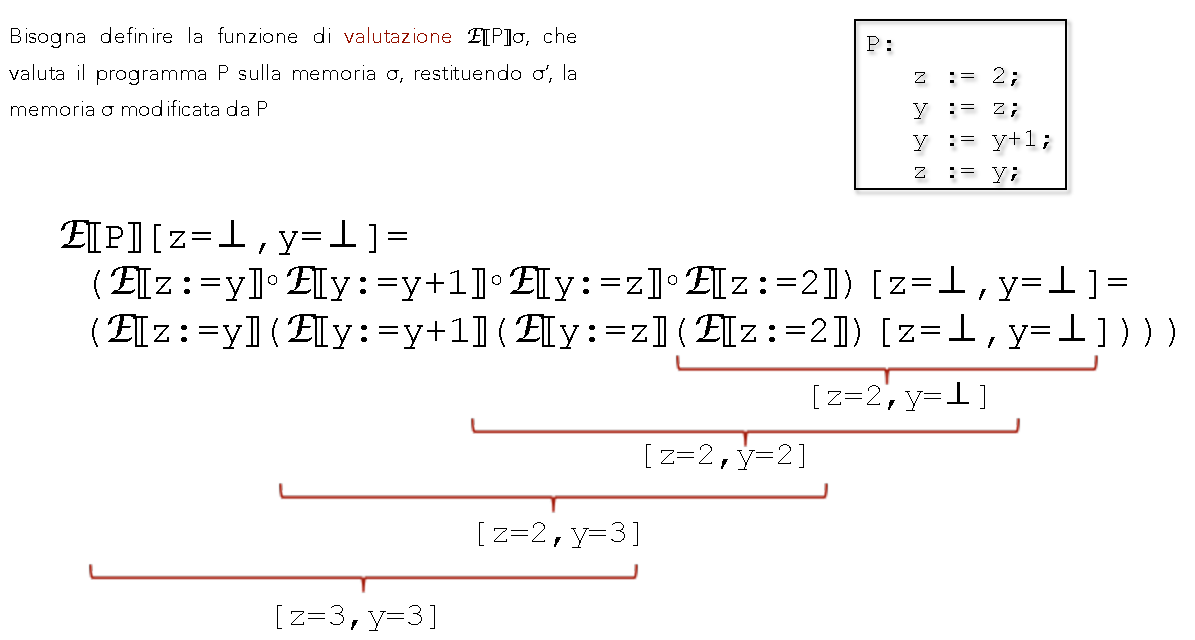
\includegraphics[scale=0.75]{immagine01.pdf}
\end{center}

\subsubsection*{Semantica assiomatica}
La semantica assiomatica consiste in un modello matematico  dei programmi basato sulla logica formale (calcolo dei predicati).

\noindent Si basa su assiomi  e regole  di  inferenza,  fornite  per  ogni  tipo  di  costrutto  del linguaggio. 

\noindent Le  espressioni  logiche  della  semantica  sono chiamate asserzioni:  
\begin{itemize}
\item[-] L’asserzione   prima   di   un   comando   (precondizione) dichiara   le   relazioni   e   i   vincoli   validi   prima dell’esecuzione del comando;
\item[-] L'asserzione che segue un comando è una post-condizione;
\item[-] Una weakest precondition è la precondizione meno restrittiva che garantisce la post-condizione.
\end{itemize}

Attraverso   queste   asserzioni,   la   semantica   assiomatica permette  di  dimostrare  proprietà  parziali  di  correttezza: quando   lo   stato   iniziale   rispetta   la   precondizione   e   il programma   termina,   allora   lo   stato   finale   soddisfa   la postcondizione.  

Poichè questo tipo di semantica considera solo gli aspetti descritti dalle pre e post condizioni, possono esistere ininiti programmi che le soddisfano, avendo però comportamenti potenzialmente diversi.

\begin{center}
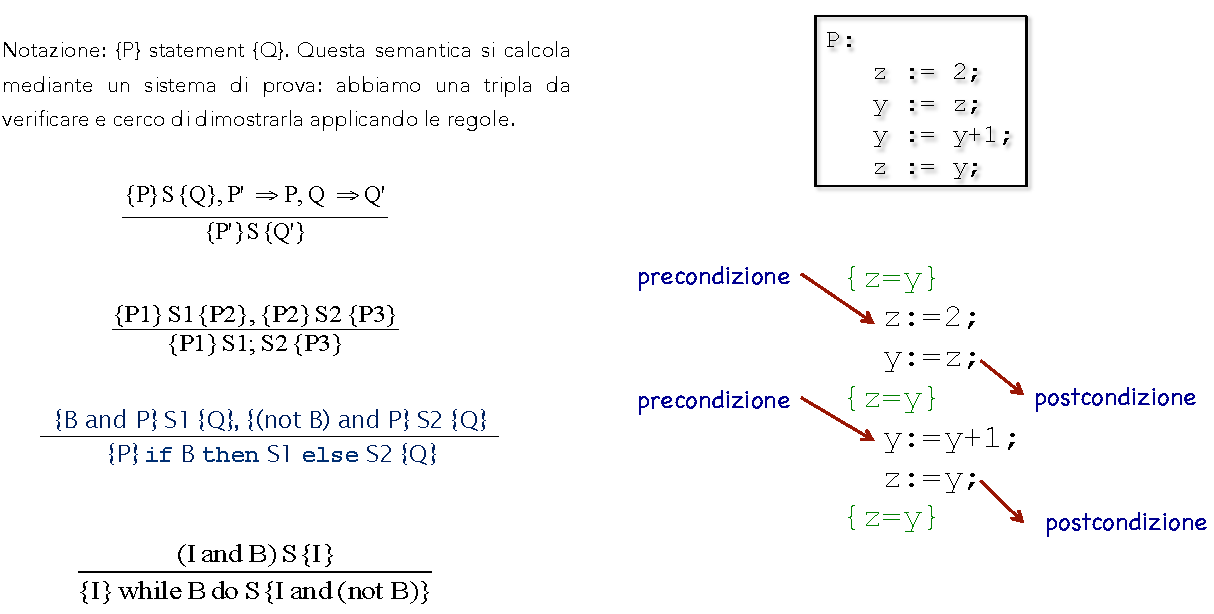
\includegraphics[scale=0.75]{immagine02.pdf}
\end{center}

\subsubsection*{Semantica operazionale}
La semantica operazionale consiste in un modello matematico  dei programmi basato sui sistemi di transizione.

Descrive   il   significato   del programma  eseguendo  i  suoi  comandi  su  una  macchina, simulata   o   reale, dove il cambiamento di stato definisce il significato del contenuto.

Per il calcolo dei risultati finali, utilizza il modello matematico dei sistemi di transizione.

\begin{center}
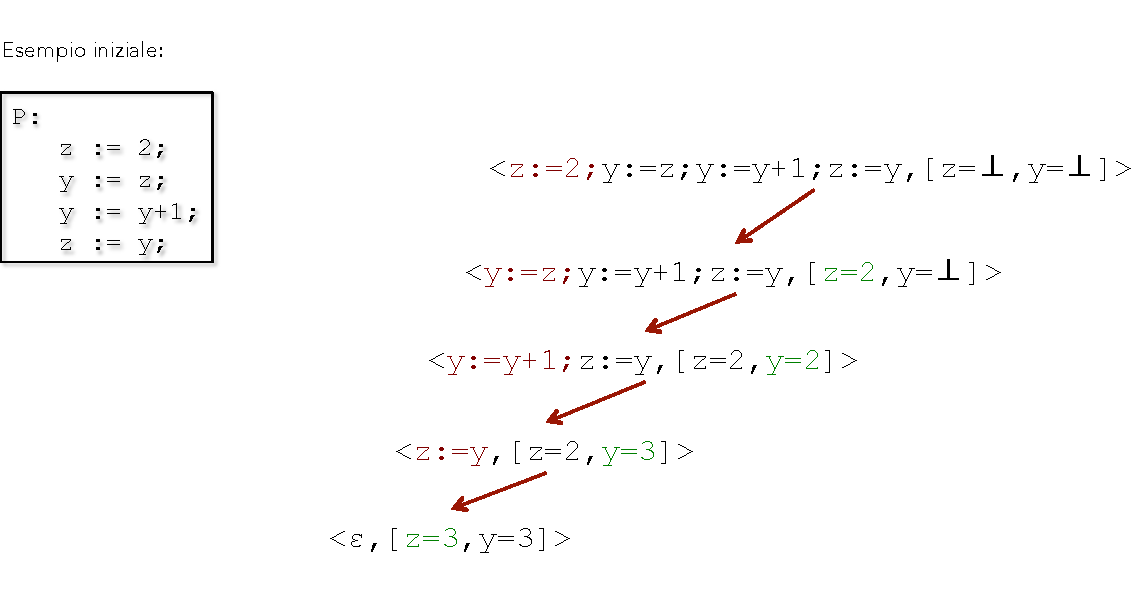
\includegraphics[scale=0.75]{immagine03.pdf}
\end{center}

\subsubsection*{Composizionalità}
La composizionalità è una proprietà della semantica necessaria  per  caratterizzare  i  comportamenti  e  significati di sistemi che possono avere infiniti elementi. Indica che il significato di ogni programma deve essere funzione del significato dei costituenti immediati. Queso principio è rispettato, di natura, dalla semantica denotazionale e assiomatica.

La composizione è molto importante per l'analisi di software di grandi dimensioni. Infatti, se la semantica su cui si basa l'analisi è composizionale, è possibili scomporre il software in moduli più piccoli, studiarli singolarmente e poi ricomporre i risultati per ottenere quello globale.



\end{document}